\documentclass[11pt]{article}
%\usepackage{cite}
\usepackage[numbers]{natbib}
\usepackage{xcolor}
\usepackage{ulem}
\usepackage{graphicx}
\usepackage{subcaption}
\usepackage{multirow}
\usepackage{booktabs}
\usepackage{amssymb}
\usepackage{tabularx} % in the preamble
\title{\textbf{Draft research question}}
%\author{Mathias Parisot}

\begin{document}
\maketitle

\section{Roadmap}

\begin{enumerate}
  \item introduction and literature study (1.5 weeks) introduction + related works
  \item draft methodology to answer research question (1 week)
  \item experiment with simple attacks (1-2 weeks)
  \item implement methodology and start experiment (3-4 weeks)
  \item \textbf{analyse results (2-3 weeks)}
  \item \textbf{write paper (2 weeks)}
  \item presentation(1-2 weeks)
\end{enumerate}

\section{Introduction}

\begin{enumerate}
	\item Machine Learning and Deep Learning description\\
Machine Learning (ML) applications have grown in popularity over the last decade. One of the most common use of ML is to train models, called classifiers, to learn a mapping function between some input data and a set of classes. A popular way of implementing such models is to use artificial neural networks. Deep Learning (DL) is the field studying neural networks containing several hidden layers. DL models require a large amount of training data and only became popular recently with the advances in hardware and algorithms allowing to process this data efficiently. Due to the huge amount of data generated by the Internet, communication data, social media websites, pictures, among others, corporations became interested in using ML models to automate some of their decision making. Because of that cloud providers such as AWS\footnote{https://aws.amazon.com/machine-learning/}, Microsoft Azure\footnote{https://azure.microsoft.com/en-us/services/machine-learning/}, Google Cloud AI\footnote{https://cloud.google.com/ai-platform} or IBM Watson\footnote{https://www.ibm.com/cloud/machine-learning} started to include ML as a Service to their offer, allowing their users to train and deploy machine learning models given they provide the dataset.\\
With the increasing amount of data generated and its use by companies to gain insights and improve their processes, governements and authorities have been trying to give control to individuals over how their data is used. An example of such action is the legal act in the European Union concerning data protection and privacy called the General Data Protection Regulation. This regulation enforces entities processing personal data to put in place measures to implement principles (see Art. 5) such as:
\begin{itemize}
	\item lawfulness, fairness and transparency
	\item purpose limitation
	\item data minimisation
	\item accuracy
	\item storage limitation
	\item integrity and confidentiality
\end{itemize}
As training ML and DL models requires dealing with plenty of data, and because such models are becoming more and more popular, companies using them need to make sure their datasets stays confidential. However, ML models are sensitive to malicious attacks. Given a classification model, once trained, it is able to label a data instance to the appropriate class by learning mapping patterns between the training dataset and the set of classes. The mapping is contained within the model parameters, in the case of a neural network it is the architecture and weight values. Therefore, an attacker knowing the parameters of a trained model, also know some information about the data it was trained on. If the data was composed of personal data, there is a potential confidentiality leak. Attacks on ML models can be classified into four categories. Model extraction attacks aim at inferring the behaviour of the target model in order to create a substitute model. A more advance feat is to create a duplicate by infering the architecture and the parameters values. Adversarial attacks aim at taking advantage of the weakness of the classification boundary of the target model in order to find craft data instances that are wrongly classified. Poisoning attacks are similiar to adversarial attacks as their goal is to also influence the prediction of the target model, however they do that by poluting the training set with malicious samples. Model Inversion attacks aim at inferring information about the training data, this can be its composition or specific properties of the dataset. 
	\item Deep Learning popularity
	\item More and more data is available
	\item Public concern about Data Privacy (talk about GDPR)
	\item ML and DL models are sensible to privacy attacks (list attacks)
	\item Complexity of models vs success of attacks 
\end{enumerate}

	Machine Learning (ML) applications have grown in popularity over the last decade. One of the most common use of ML is to train models, called classifiers, to learn a mapping function between some input data and a set of classes. A popular way of implementing such models is to use artificial neural networks. Deep Learning (DL) is the field studying neural networks containing several hidden layers. DL models require a large amount of training data and only became popular recently with the advances in hardware and algorithms allowing to process this data efficiently. Due to the huge amount of data generated by the Internet, communication data, social media websites, pictures, among others, corporations became interested in using ML models to automate some of their decision making. Because of that cloud providers such as AWS\footnote{https://aws.amazon.com/machine-learning/}, Microsoft Azure\footnote{https://azure.microsoft.com/en-us/services/machine-learning/}, Google Cloud AI\footnote{https://cloud.google.com/ai-platform} or IBM Watson\footnote{https://www.ibm.com/cloud/machine-learning} started to include ML as a Service to their offer, allowing their users to train and deploy machine learning models given they provide the dataset.\\
With the increasing amount of data generated and its use by companies to gain insights and improve their processes, governements and authorities have been trying to give control to individuals over how their data is used. An example of such action is the legal act in the European Union concerning data protection and privacy called the General Data Protection Regulation. This regulation enforces entities processing personal data to put in place measures to implement principles (see Art. 5) such as:
\begin{itemize}
	\item lawfulness, fairness and transparency
	\item purpose limitation
	\item data minimisation
	\item accuracy
	\item storage limitation
	\item integrity and confidentiality
\end{itemize}
As training ML and DL models requires dealing with plenty of data, and because such models are becoming more and more popular, companies using them need to make sure their datasets stays confidential. However, ML models are sensitive to malicious attacks. Given a classification model, once trained, it is able to label a data instance to the appropriate class by learning mapping patterns between the training dataset and the set of classes. The mapping is contained within the model parameters, in the case of a neural network it is the architecture and weight values. Therefore, an attacker knowing the parameters of a trained model, also know some information about the data it was trained on. If the data was composed of personal data, there is a potential confidentiality leak. Attacks on ML models can be classified into four categories. Model extraction attacks aim at inferring the behaviour of the target model in order to create a substitute model. A more advance feat is to create a duplicate by infering the architecture and the parameters values. Adversarial attacks aim at taking advantage of the weakness of the classification boundary of the target model in order to find craft data instances that are wrongly classified. Poisoning attacks are similiar to adversarial attacks as their goal is to also influence the prediction of the target model, however they do that by poluting the training set with malicious samples. Model Inversion attacks aim at inferring information about the training data, this can be its composition or specific properties of the dataset. 
    Several kinds of model inversion attacks exist with different goals: the attacker could want to determine whether a data instance was used for training (membership inference)\cite{Shokri2017, Salem2019}, reconstruct a representative of a particular class of the training set \cite{Fredrikson2015}, or infer hidden properties of the training set (property inference)\cite{Ganju2018}.\\
    
    (TODO): The implementation of the GDPR in 2018 has put a question on whether those kinds of models are compliant (\textcolor{blue}{\textit{\underline{question}: can it be argued that if the model learns more information than it needs, then Art.5.1.c - data minimization applies?} I still need to write this part}).\\
    
Membership inference attacks work the following way: given a data point, determine whether it was used to train the given model. The issue with such attacks is they are not always applicable in real-life settings as the attacker needs to get a copy of one of the training data before determining whether it belonged to the training set. Inversion model attacks operate such that, for a classifier, for example, a class representative can be created. While they are impressive for face recognition models, they only build the “average” representation of the class and do not work well if the data instances are not similar.
Property Inference Attacks (PIA) aim at inferring properties learned by the model that are independent of the characteristics of the class the model is trained to recognize. There have been fewer studies on this kind of attack, according to \citet{He2019} only 4 papers were published on model inversion attacks against 10 for membership inference attacks. In \cite{Ganju2018} the authors identify the invariance of fully connected neural networks to node permutation as a limiting factor of PIA efficiency and show that using a Deep Set architecture \cite{zaheer2017deep} is an effective way to tackle this limitation. In \cite{Melis2019} the authors successfully perform PIA in a collaborative learning setting where the attacker is one of the members.\\

The kind of model used has an impact on the kind of attacks that can be used on it (\textcolor{blue}{I still need to do that. \textit{\underline{remark}: I probably need to include a source here, it is a bit of a strong claim.}}). As computer vision and natural language processing popularity increases, more complex neural network architectures are created even if their vulnerability to privacy attacks is still not fully determined \cite{He2019}. None of the current work studied the relationship between the depth and width of a deep neural network and its sensibility to PIA. \citet{Geiping2020} analyzed the effect of model architecture on sensibility to model inversion attacks on non-sensible data (cars, animals).\\


\textbf{In case of a trained Neural Network, are sensitive properties of the underlying dataset at risk due to property inference attacks, and if so, how does that risk relate to the architecture of the model such as depth and width?}
\begin{itemize}
\item{\textcolor{blue}{How does the sensibility to property inference attacks change with changes in depth and width of deep neural networks?}}
\item{\textcolor{blue}{Does it affect compliance with the GDPR concerning the processing of sensitive data?}}
\item{\textcolor{blue}{Question: do I still need to specify the secondary questions when the initial research question is detailed? Or should I make the research question broader and the secondary questions more detailed?}}
\end{itemize}

\section{\textcolor{blue}{Related Works}}

\citet{Zhang2019} present a model inversion attack using Generative Adversarial Networks. They study and theoretically prove the relation between a model predictive power and its vulnerability to model inversion attacks. The influence of the predictive power of a model is a hint that more complex models, which should have greater predictive power, should also be more sensitive to model inversion attacks. However, the result of \citet{Zhang2019} was not proven for PIAs. We also focus more specifically on the architecture of the target model.\\
Several studies \cite{Melis2019, Wang2019} performed PIAs in a federated learning setup which allows multiple clients to train a common model without the need to share data. Only the weights and the gradients after each round of training are exchanged which can help tackle privacy issues. \citet{Melis2019} managed to infer properties that hold for a subset of the training data and that are independent of the property the target model aims at predicting. Because it is performed in a federated learning setting, the attacker has access to the architecture and weights of the model. Moreover, the attack is performed during the training or, at least, requires the model updates that are exchanged between participants. The attack we focus on does not require the gradients' values after each round of training. We also target properties that are true for the whole dataset and not only a subset of it. \citet{Wang2019} propose three kinds of PIAs: class sniffing, quantity inference, and whole determination. Class sniffing detects whether a training label is present within a training round, quantity inference determines how many clients have a given training label in their dataset, whole determination infers the global proportion of a specific label. All of those attacks are extracting properties related to classification labels, and therefore to the main classification task. We focus on properties that are unrelated to the task of the target model.\\
\citet{Geiping2020} study model inversion attacks and analyze the effects of the architecture of the target model on the difficulty of reconstructing input images. They investigate attacks on networks with various widths and depths and found that the width has the greatest influence on the quality of the reconstruction. Their study does not consider PIAs and is restricted to federated learning as they use the gradients' values in their attack.\\
\citet{Ateniese2015} describe the first PIA attack using meta-classifiers, the methodology of the attack we use in our research. Their research is not focussed on the privacy leakage caused by such attack but rather on the impact of the training set properties on the model performance with the commercial benefits that it represents. Moreover, they attack models implemented via Support Vector Machines and Hidden Markov Models using a binary tree meta-classifier but do not experiment with deep neural network models. \citet{Ganju2018} extend the research of \citet{Ateniese2015} to neural networks and notice that a limitation of PIA performance is due to a property of fully connected networks called invariance to weights permutations within the same layer. They propose two successful strategies to reduce the impact of this property: converting a neural network to a canonical form and using a deep set architecture. They use a pre-trained network to generate an embedding which they feed as input to their target neural network. They do not study the influence of the architecture of the model on the attack performance.\\


\section{\textcolor{blue}{Background}}

\subsection{\textcolor{blue}{Deep Learning model}}
(TODO)

\section{Methodology}
To answer the research question, we will perform several PIAs on different target model architectures. For each architecture, we will train attack models and evaluate their performance. This section presents the attack strategy alongside with the assumptions about the target model. \\

\subsection{Threat model}

We suppose the target model is a deep neural network classifier. The training dataset of the classifier contains sensitive data according to the definition used in article 9.1 of the GDPR. The attack is performed in a white-box setting, which means the attacker has access to the full architecture and parameter values of the model. While a white-box model may be seen as a big assumption in some scenario, it is realistic in ours as it is common in some machine learning paradigms such as Federated Learning \cite{shokri2015privacy} where the clients, and sometimes the server, have full knowledge of the model, and access is only restricted to the dataset. Moreover, model extraction attacks have been done to perform adversarial attacks on deep neural netowrks in a black-box setting. The attackers managed to create a substitute model with a similiar decision boundary as the target model allowing them to achieve larger than 88\% missclassification rates in real-world settings \cite{DBLP:journals/corr/PapernotMGJCS16}. The specificities of a model extraction attack fall out of the scope of this study. In here, we assume the attacker has access to the model architecture and parameter values, independent of how this knowledge was obtained. The goal of the attacker is to infer general information about the training dataset such as the proportion of the training data having a property unrelated to the main classification task of the model.

\subsection{Attack Strategy: Property Inference Attack}
In this subsection, we present the general idea of the attack we used in our experiments. We focus on PIAs which goal is to extract general information about the training dataset of the target model. The information is often presented using a property $P$ which can be true or false. For example, if the dataset used contains images of cars, $P$ could be: \textit{the dataset includes 20\% of images of Ferrari}, or any other brand. We can transform a PIA into a classification task where the goal is as follows: given a trained model, determine whether it was trained using a dataset presenting the given target property $P$. It is then possible to train a classifier to solve the previous classification task. Such a model is called a meta-classifier because the dataset on which it is trained on is composed of models which are themselves classifiers.

The PIA used in this paper is the baseline attack presented in \cite{Ganju2018}. The main idea is to use a meta-classifier to train an attack model $M_a$ which takes as input the weights of a trained model and outputs the probability that the target property $P$ is true for the training set of the input model. Once the attack model is trained, the attacker can give it the target model $M_t$ as input and know whether the property $P$ is true for the dataset used to train the target model. The main problem is then to find enough trained models to use as the training set for the attack model $M_a$. This is solved by using shadow models with the same architecture as the target model $M_t$. The attacker trains $k$ shadow models ($M_{s1}$ ... $M_{sk}$) on k datasets ($D_1$ ... $D_k$ respectively) specifically crafted to contain or not the target property $P$. The general overview of the attack is described in Figure \ref{pia_diagram}.\\
This PIA is the baseline attack presented in \cite{Ganju2018}. This paper is not focused on the PIA itself but rather on the behavior of the PIA performed on models with different complexities. \\ %We discuss the details of the target models and their complexities in section 2.\\

\begin{figure}[h]
    \centering
    \begin{minipage}{\textwidth}
        \centering
        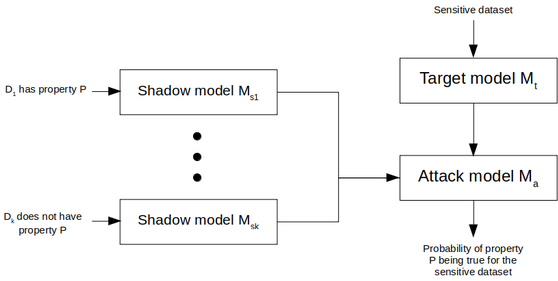
\includegraphics[width=0.99\textwidth]{pia_diagram2.png} % first figure itself
        \caption{Property Inference Attack using a meta-classifier and a dataset of shadow models.}
        \label{pia_diagram}
    \end{minipage}\hfill
\end{figure}

\section{Experimental Setup}

In this section, we describe the experimental settings: the dataset, the architectures of the target and attack models, and the evaluation metrics. The experiments were performed on a laptop with an Intel i7-8750H (2.20GHz) and 8GB RAM. The operating system is Ubuntu 20.04. The training of the shadow models and the attack models were both done using Pytorch and an Nvidia Quadro P600 GPU.\\

\subsection{Datasets}

CelebFaces Attributes (CelebA) \cite{liu2015faceattributes} is a face attributes dataset containing more than 200 000 images of more than 10 000 celebrities taken from online. The images are labeled using 40 physical attributes such as hair color, smiling, wearing a hat. We use the dataset to train the shadow models $M_s$ to detect whether the person has their mouth open using the \textit{Mouth\_Open} attribute. Although this might seem like a unimportant cassification task, in the time of a COVID-19 pandemic, there have been questions about how technology can help the fight against the virus. Some governements are trying to track the persons who have been in contact with a contaminated subject using mobile applications\footnote{https://www.nature.com/articles/d41586-020-01264-1}, in some countries facial masks became compulsory in public places and companies are marketing mask-detection software\footnote{https://www.theverge.com/2020/5/7/21250357/france-masks-public-transport-mandatory-ai-surveillance-camera-software}. Detecting whether someone has their mouth open can be associated with detecting whether someone is wearing a face mask. The property targeted by the attacker is the balance of the gender proportion of the training set using the \textit{Male} attribute. The images are centered and resized to 64 by 64 pixels.\\

\subsection{Shadow Models}
The shadow models are trained to differentiate between images of persons with and without their mouth open.
However, the goal of the attacker is to infer whether the training set of a given model was composed of an unbalanced number of images representing males. The targeted property is a biometric data and is classified as sensitive data according to the GDPR. For a given model, the property $P$ can be formalized as follow: \textit{P is true when the training set of the model is composed of 70\% or more images containing males, otherwise, P is false}. It is important to note that $P$ is not related to the classification task of the model and that the target model does not use, at any time during training, the gender attribute.\\

The shadow models $M_{s_k}$ must have the same architecture as the targeted model, and be trained to a reasonable level of accuracy for the network to retain some information about the training set. For example, all of our shadow models have at least 85\% accuracy on the mouth open classification task when the baseline distribution of the dataset is 51.7\%. For the attack to be effective, a large number of shadow models need to be trained. For each target model architecture, we constructed 1800 unique training sets of images from CelebA, one for each of the 1800 shadow models. The computational cost of such training is not negligible so we decide to lower it by reducing the size of the shadow datasets $D_{s_k}$ to 2000 different images each randomly selected from the test set of \textit{CelebA}. Out of the 1800 shadow models, 900  were trained on datasets presenting the property $P$ and 900 without. For each dataset, the exact proportion of males was randomly taken from a uniform distribution.\\

The shadow model architectures are composed of up to 9 layers which can each be of three kinds: convolution layers, pooling layers, fully connected layers. The description of each layer is presented in Table \ref{layer_description}. We trained 9 architectures ($A_1$ to $A_9$) which are presented in Table \ref{shadow_architecture}. The models take as input 64 by 64 RGB face images and output the probability of each picture representing a person with a mouth open. All the networks are composed of 1 to 3 convolution layers, each followed by a max-pooling layer with a ReLU activation, and 1 to 3 fully connected layers with a ReLU activation. The shadow models were trained using the Mean Squared Error loss and the Adam optimizer with a learning rate of 0.001 during 50 epochs.\\

\begin{table}[h!]
\centering
\begin{tabular}{@{}ll@{}}
\toprule
Layer              & Description       \\ \midrule
Convolution 1     & 6 filters 5x5     \\
Max-pool          & 2x2, ReLU         \\
Convolution 2     & 16 filters 5x5    \\
Max-pool          & 2x2, ReLU         \\
Convolution 3     & 32 filters 5x5    \\
Max-pool          & 2x2, ReLU         \\
Fully-Connected 1 & 120 neurons, ReLU \\
Fully-Connected 2 & 84 neurons, ReLU  \\
Fully-Connected 3 & 1 neuron          \\ \bottomrule
\end{tabular}
\caption{Description of the different layers used in the shadow architectures presented in Table \ref{shadow_architecture}.}
\label{layer_description}
\end{table}



\begin{table}[h!]
\centering
\begin{tabular}{@{}lccccccccc@{}}
\toprule
    & Conv 1               & Max-pool             & Conv 2               & Max-pool             & Conv 3               & Max-pool             & FC 1                 & FC 2                 & FC 3                 \\ \midrule
    & \multicolumn{1}{l}{} & \multicolumn{1}{l}{} & \multicolumn{1}{l}{} & \multicolumn{1}{l}{} & \multicolumn{1}{l}{} & \multicolumn{1}{l}{} & \multicolumn{1}{l}{} & \multicolumn{1}{l}{} & \multicolumn{1}{l}{} \\
A 1 & \checkmark           & \checkmark           & \checkmark           & \checkmark           & \checkmark           & \checkmark           & \checkmark           & \checkmark           & \checkmark           \\
A 2 & \checkmark           & \checkmark           & \checkmark           & \checkmark           & \checkmark           & \checkmark           & \checkmark           &                      & \checkmark           \\
A 3 & \checkmark           & \checkmark           & \checkmark           & \checkmark           & \checkmark           & \checkmark           &                      &                      & \checkmark           \\
A 4 & \checkmark           & \checkmark           & \checkmark           & \checkmark           &                      &                      & \checkmark           & \checkmark           & \checkmark           \\
A 5 & \checkmark           & \checkmark           & \checkmark           & \checkmark           &                      &                      & \checkmark           &                      & \checkmark           \\
A 6 & \checkmark           & \checkmark           & \checkmark           & \checkmark           &                      &                      &                      &                      & \checkmark           \\
A 7 & \checkmark           & \checkmark           &                      &                      &                      &                      & \checkmark           & \checkmark           & \checkmark           \\
A 8 & \checkmark           & \checkmark           &                      &                      &                      &                      & \checkmark           &                      & \checkmark           \\
A 9 & \checkmark           & \checkmark           &                      &                      &                      &                      &                      &                      & \checkmark           \\
    & \multicolumn{1}{l}{} & \multicolumn{1}{l}{} & \multicolumn{1}{l}{} & \multicolumn{1}{l}{} & \multicolumn{1}{l}{} & \multicolumn{1}{l}{} & \multicolumn{1}{l}{} & \multicolumn{1}{l}{} & \multicolumn{1}{l}{} \\ \bottomrule
\end{tabular}
\caption{Layer-level description of each shadow architectures. The detailed description of the parameters in each layer is presented in Table \ref{layer_description}.}
\label{shadow_architecture}
\end{table}


\subsection{Attack Model and Evalution}
The attack model classifies shadow models as models trained on a dataset presenting the property $P$ or not. The dataset used is composed of the 1800 shadow models and is split into training (1500 shadow models), validation (100 models), and test sets (200 models). The attack model is a deep neural network that was tunned using the validation set and finally evaluated on the test set. The inputs of the attack model are the flattened weights of the model it is trying to classify as having the property $P$ or not. Therefore, a shadow model architecture with a larger number of parameters induces a wider input layer for the attack model. We created 10 attack models for each shadow model architecture and present the average performance across the 10 repetitions.\\

\begin{table}[h!]
\centering
\begin{tabular}{@{}ll@{}}
\toprule
Name              & Description       \\ \midrule
Fully-Connected 1 & 10 neurons, ReLU  \\
Fully-Connected 2 & 10 neurons, ReLU  \\
Fully-Connected 3 & 5 neurons, ReLU  \\
Fully-Connected 4 & 1 neuron          \\ \bottomrule
\end{tabular}
\caption{Architectures of the attack model. [TODO]}
\label{attack_architecture}
\end{table}

\section{Results and Discussions}
Accuracies of the PIAs on each of the architectures of the target model are presented in Figure \ref{accuracies}. The larger/complex the target model is the more successful the PIA is. TODO

\begin{figure}[h!]
    \centering
    \begin{minipage}{\textwidth}
        \centering
        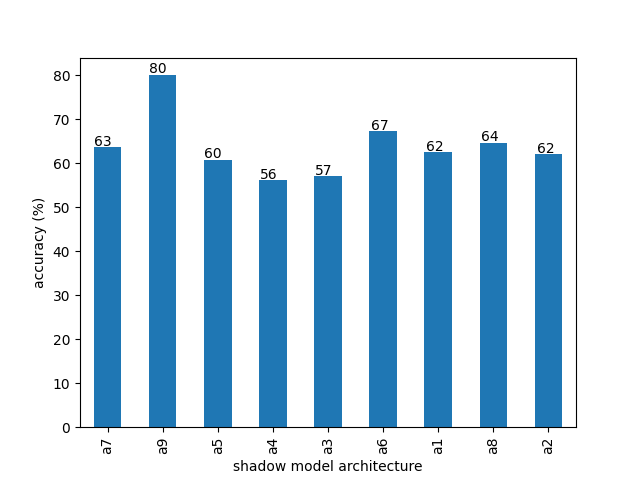
\includegraphics[width=0.99\textwidth]{accuracies.png} % first figure itself
        \caption{Accuracies of the attack of each architecture of target models. The architecture are ordered by increasing number of parameters.}
        \label{accuracies}
    \end{minipage}\hfill
\end{figure}


\newpage
%\renewcommand\bibliographytypesize{\small}
%\bibliographystyle{alpha}
%\bibliography{references.bib}{}
\bibliographystyle{unsrtnat}
\bibliography{references.bib}


\end{document}
